\documentclass[10pt]{beamer}

\usepackage[utf8]{inputenc}
\beamertemplatenavigationsymbolsempty

%\usetheme{default}
%\usetheme{AnnArbor}
\usetheme{Antibes}
%\usetheme{Bergen}
%\usetheme{Berkeley}
%\usetheme{Berlin}
%\usetheme{Boadilla}
%\usetheme{CambridgeUS}
%\usetheme{Copenhagen}
%\usetheme{Darmstadt}
%\usetheme{Dresden}
%\usetheme{Frankfurt}
%\usetheme{Goettingen}
%\usetheme{Hannover}
%\usetheme{Ilmenau}
%\usetheme{JuanLesPins}
%\usetheme{Luebeck}
%\usetheme{Madrid}
%\usetheme{Malmoe}
%\usetheme{Marburg}
%\usetheme{Montpellier}
%\usetheme{PaloAlto}
%\usetheme{Pittsburgh}
%\usetheme{Rochester}
%\usetheme{Singapore}
%\usetheme{Szeged} 
%\usetheme{Warsaw}


%\usecolortheme{albatross}
%\usecolortheme{beaver}
%\usecolortheme{beetle}
%\usecolortheme{crane}
%\usecolortheme{dolphin}
%\usecolortheme{dove}
%\usecolortheme{fly}
%\usecolortheme{lily}
%\usecolortheme{orchid}
%\usecolortheme{rose}
%\usecolortheme{seagull}
%\usecolortheme{seahorse}
%\usecolortheme{whale}
%\usecolortheme{wolverine}

%\setbeamertemplate{footline}%\setbeamertemplate{footline}[page number]
%\setbeamertemplate{navigation symbols}{}}

\usepackage{graphicx}
\usepackage{booktabs}

\usepackage{subcaption}
\usepackage{lmodern}
\usepackage{amsmath}
\usepackage{amsfonts}
\usepackage{amssymb}
\usepackage{hyperref, url}
\usepackage{tikz, pgfplots}
\usepackage[ruled,vlined,linesnumbered,noend]{algorithm2e}

\newcommand{\dom}{\mathrm{dom}}
\newcommand{\xf}{\mathbf{x}}
\newcommand{\yf}{\mathbf{y}}
\newcommand{\wf}{\mathbf{w}}
\newcommand{\uf}{\mathbf{u}}
\newcommand{\vf}{\mathbf{v}}
\newcommand{\kf}{\mathbf{k}}
\newcommand{\Tf}{\mathbf{T}}
\newcommand{\Qc}{\mathcal{Q}}
\newcommand{\Uc}{\mathcal{U}}
\newcommand{\Pc}{\mathcal{P}}
\newcommand{\R}{\mathbb{R}}
\newcommand{\E}{\mathbb{E}}
\newcommand{\N}{\mathbb{N}}

\newcommand{\idx}{\varphi}
\newcommand{\varidx}{\psi}
\newcommand{\move}[3]{#1_{#2\rightarrow #3}}
\newcommand{\image}{\mathrm{image}}
\newcommand{\minimize}{\text{minimize}}
\renewcommand{\iff}{\quad\text{iff}\quad}


\DeclareMathOperator*{\argmin}{\arg\min}
\DeclareMathOperator*{\argmax}{\arg\max}

%----------------------------------------------------------------------------------------
%	TITLE PAGE
%----------------------------------------------------------------------------------------

\title[A Local Search Algorithm for Cubic Clustering]{A Local Search Algorithm for Cubic Clustering}
\author{Hans Harder}\institute[TU Dresden]{
TU Dresden \\\medskip
\textit{hans.harder@mailbox.tu-dresden.de}}
\date{}



\begin{document}

\begin{frame}
\titlepage\end{frame}

\begin{frame}
\frametitle{Overview}
\tableofcontents
\end{frame}

\section{Problem}
\begin{frame}{Notation / Sets}
    \begin{itemize}
        \item $k$-ary subsets of $V$
        \begin{align*}
            \binom{V}{k} = \{ \{ v_1, \dots, v_k \} \subseteq V : v_1, \dots, v_k \text{ pairwise distinct}\}
        \end{align*}
        \item $X_V$ is the set of partitions of $V$
        \item for $\Pi \in X_V$ and $v \in V$, then $[v]_\Pi$ denotes the set in $\Pi$ that contains $v$ (e.g. for $\Pi = \{ \{ 1,2 \}, \{3\}\}$ then $[1]_\Pi = \{1,2\}$)
    \end{itemize}
\end{frame}

\begin{frame}{Notation / Random Variables}
    \begin{itemize}
        \item random variables $\xf,\yf,\dots$ and distributions $\Qc, \Uc,\dots$
        \item random variable ``distributed as'' $\xf \sim \Qc$
        \item uniform distribution over a finite set $A$: $\Uc(A)$
        \item domain of a random variable $\xf$: $\dom(\xf)$ (e.g. $\dom(\xf) = \R$)
        \item expected value for $\xf \sim \Qc$ and $f : \dom(\xf) \rightarrow \R$ and $\dom(\xf)$ finite: $$\E_{\xf \sim \Qc}\left[ f(\xf) \right] = \sum_{x \in \dom(\xf)} \Qc(x) f(x)$$
    \end{itemize}
\end{frame}

\subsection*{Problem Statement}
\begin{frame}{Problem Statement}
    \textbf{Input:} finite set $V$, functions $c,c': \binom{V}{3} \rightarrow \R$ \\
    \textbf{Output:} partition $\Pi^*$ of $V$ such that $$ \Pi^* = \argmin_{\Pi \in X_V} \sum\nolimits_{T \in \binom{V}{3}} \ell(T, \Pi) $$
    where $$ \ell(\{u,v,w\}, \Pi) = \begin{cases}
        c'(\{u,v,w\}) & [u]_\Pi = [v]_\Pi = [w]_\Pi \\
        c(\{u,v,w\}) &  [u]_\Pi, [v]_\Pi, [w]_\Pi \text{ pairwise distinct} \\
        0 & \text{otherwise}
    \end{cases} $$
    \pause
    \textbf{Intuition}
    \begin{itemize}
        \item $c'$ adds penalty/reward when $u,v,w$ are in the same set 
        \item $c$ adds penalty/reward when $u,v,w$ are in different sets 
    \end{itemize}
\end{frame}

\subsection*{Local Search}
\begin{frame}{Local Search}
    \textbf{Objectives}
    \begin{itemize}
        \item defining a data structure for representing partitions
        \item defining a neighbourhood for every partition
        \item defining a search algorithm (e.g. hill climbing)
    \end{itemize}
    \pause 
    \textbf{Difficulties}
    \begin{itemize}
        \item if $V$ is large, computing the costs in $O(|V|^3)$ is problematic
        \item even runtimes in $O(|V|^2)$ are prohibitive in this case\footnote{if only the reduced cost is computed}
        \item the neighbourhood for a partition might become large as well
    \end{itemize}
\end{frame}

\subsection*{Objective}
\begin{frame}{Objective}
    There are many local search algorithms that work equally well.
    %All local search algorithms work equally well if all cost structures are equally likely\footnote{This is the result of the ``No free lunch theorem(s) for search'' (Wolpert et al., \cite{wolpert1995no}) -- since we are not given any \emph{a priori} information on the cost-structures, we might as well assume this (however, one might argue that this is not the case in praxis and that most cost-structures are generally).}.
    \textbf{Therefore:} focus on shared difficulties.
    \begin{itemize}
        \item efficient representation (memory-wise) of partitions
        \item efficient transformations (from partitions to their neighbours)
        \item efficient enumeration of the neighbourhood
    \end{itemize}
    \textbf{and for large $V$'s}
    \begin{itemize}
        \item efficient sampling of neighbours from the neighbourhood
        \item approximation of the reduced costs
    \end{itemize}
\end{frame}

\section{Data Structure}
\subsection*{Basic Idea}
\begin{frame}{Basic Idea}
    \textbf{Indexing}
    \begin{itemize}
        \item represent a partition by a mapping $\idx: V \rightarrow \{ 1,\dots, n \}$ where $|V| = n$ (this can be implemented by an array of length $|V|$)
        \item the \emph{equivalence kernel}\footnote{see, e.g. \url{http://en.wikipedia.org/wiki/equivalence_relation}.} of $\idx$ is the equivalence relation $\sim_\idx$ where $u \sim_\idx v$ iff $\idx(u) = \idx(v)$.
        \item $\sim_\idx$ yields a partition $\Pi(\idx)$ of $V$.
        \item we say that the \emph{indexing} $\idx$ \emph{induces} $\Pi(\idx)$.
    \end{itemize}
    \pause
    \textbf{Pro:} memory linear in $|V|$, and changing the assigned index of a $v \in V$ can be done in $O(1)$. \\
    \textbf{Con:} there are multiple ways of representing the same partition through such an indexing.
\end{frame}

\subsection*{Example Indexing}
\begin{frame}{Example Indexing}
    \begin{figure}
        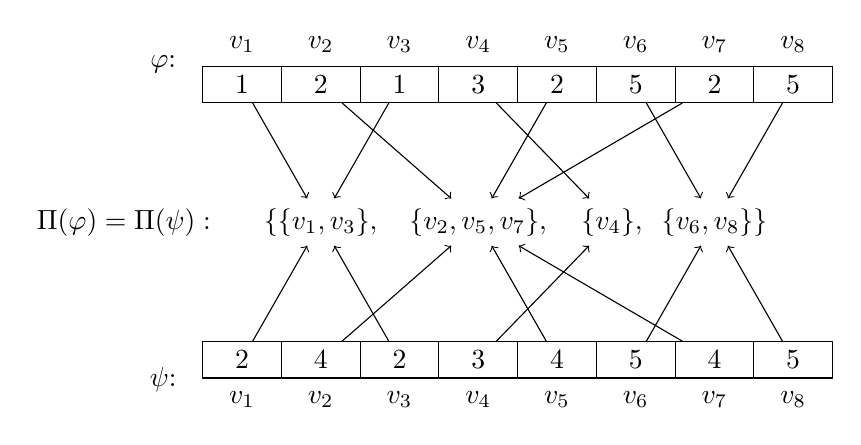
\begin{tikzpicture}
            \node at (0,1) {$\idx$:};
            \node at (-0.5,-1) {$\Pi(\idx)=\Pi(\varidx):$};
            \foreach \x\val in {1/1,2/2,3/1,4/3,5/2,6/5,7/2,8/5} {
                \node at (\x,1.25) {$v_\x$};
                \node[draw, minimum width=1cm] (u\x) at (\x,0.75) {$\val$};
            }

            \node at (0,-3) {$\varidx$:};
            \foreach \x\val in {1/2,2/4,3/2,4/3,5/4,6/5,7/4,8/5} {
                \node at (\x,-3.25) {$v_\x$};
                \node[draw, minimum width=1cm] (w\x) at (\x,-2.75) {$\val$};
            }

            \node (n1) at (2,-1) {$\{ \{ v_1, v_3 \},$};
            \node (n2) at (4,-1) {$\{ v_2, v_5, v_7 \},$};
            \node (n3) at (5.7,-1) {$\{ v_4 \},$};
            \node (n4) at (7,-1) {$\{ v_6, v_8 \} \}$};

            \foreach \v in {u,w} {
                \draw[->] (\v1) -- (n1);
                \draw[->] (\v3) -- (n1);
                \draw[->] (\v2) -- (n2);
                \draw[->] (\v5) -- (n2);
                \draw[->] (\v7) -- (n2);
                \draw[->] (\v4) -- (n3);
                \draw[->] (\v6) -- (n4);
                \draw[->] (\v8) -- (n4);
            }
        \end{tikzpicture}
    \end{figure}
    $\idx$ and $\varidx$ are different, but yield the same partition.
\end{frame}

\subsection*{Neighbourhood Enumeration}
\begin{frame}{Neighbourhood of an Indexing}
    we define the following transformation:
    \begin{align*}
        \move{\idx}{v}{k}(u) = \begin{cases}
            k & u = v \\
            \idx(v) & u \neq v
        \end{cases}
    \end{align*}
    which ``moves'' an element $v$ to a (new) index $k$. 
    \par \hrulefill \par 
    The neighbourhood of a partition $\Pi(\idx)$ is defined as the set $$Ne(\Pi(\idx)) = \{  \Pi(\move{\idx}{w}{k}) : w \in V, 1 \leq k \leq n, \Pi(\move{\idx}{w}{k}) \neq \Pi(\idx) \}.$$
\end{frame}

\begin{frame}
    The neighbourhood of a partition $\Pi(\idx)$ is defined as the set $$Ne(\Pi(\idx)) = \{  \Pi(\move{\idx}{w}{k}) : w \in V, 1 \leq k \leq n, \Pi(\move{\idx}{w}{k}) \neq \Pi(\idx) \}.$$
    \par \hrulefill \par 
    \textbf{Open Questions.}
    We want to find an efficient enumeration of possible ``moves'' $(w_1,k_1),\dots,(w_m,k_m) \in V \times \{1,\dots,n\}$ such that
    \begin{itemize}
        \item we do not enumerate ``too much'', i.e. $\Pi(\move{\idx}{w_1}{k_1}),\dots,\Pi(\move{\idx}{w_m}{k_m})$ are all pairwise distinct,
        \item all neighbours occur somewhere in this enumeration, i.e. if $\Pi \in Ne(\Pi(\idx))$, then $\Pi = \Pi(\move{\idx}{w_i}{k_i})$ for a $(w_i,k_i)$, 
        \item we do not enumerate $\Pi(\idx)$ itself, i.e. $\Pi(\move{\idx}{w_i}{k_i}) \neq \Pi(\idx)$ for all $(w_i,k_i)$.
    \end{itemize} 
\end{frame}

\begin{frame}
    \begin{figure}
        \scalebox{0.7}{
        \begin{algorithm}[H]
            \SetAlgoLined
            \DontPrintSemicolon
            \KwIn{Set of vertices $V$ with indexing $\idx$}
            \KwResult{Sequence of moves $(w_1,k_1),\dots,(w_m,k_m)$ }
            Let $<$ be some linear order on $V$ \label{alg:moveenum:l1} \;
            Let $\mathcal{N} := \{1,\dots,n\}\backslash \image(\idx)$  \label{alg:moveenum:l2} \;
            \ForAll{vertices $w \in V$}{  \label{alg:moveenum:l3}
                \ForAll{$\idx(v) \in \image(\idx) \backslash \{ \idx(w) \}$}{  \label{alg:moveenum:l4}
                    \uIf{$[w]_\idx = \{ w, u, \dots \}$ or $[v]_\idx  = \{ v, s, \dots \}$}{  \label{alg:moveenum:l5}
                        enumerate $(w, \idx(v))$  \label{alg:moveenum:l6} \;
                    }\uElseIf{$[w]_\idx = \{ w \}$ and $[v]_\idx = \{ v \}$ and $w < v$}{ \label{alg:moveenum:l7}
                        enumerate $(w, \idx(v))$  \label{alg:moveenum:l8} \;
                    }
                }
                \uIf{$[w]_\idx = \{ w, u, v, \dots \}$ or $([w]_\idx = \{w,u\}$ and $w < u)$}{  \label{alg:moveenum:l9}
                    Let $k \in \mathcal{N}$  \label{alg:moveenum:l10} \;
                    enumerate $(w, k)$  \label{alg:moveenum:l11} \;
                }
            }
            \caption{\textsc{Move-Enumeration}} \label{alg:moveenum}
        \end{algorithm}
        }
    \end{figure}
\end{frame}

\begin{frame}
    Algorithm \textsc{Move-Enumeration} has indeed the wanted properties:
    \begin{block}{Pairwise Distinctiveness}
        $\Pi(\move{\idx}{w_i}{k_i}) \neq \Pi(\move{\idx}{w_j}{k_j})$ for all $1 \leq i < j \leq n$.
    \end{block}
    \begin{block}{Completness}
        for all $\Pi \in Ne(\Pi(\idx))$, there is $1 \leq i \leq m$ such that $\Pi = \Pi(\move{\idx}{w_i}{k_i})$.
    \end{block}
    \begin{block}{No self-neighbour}
        $\Pi(\idx) \neq \Pi(\move{\idx}{w_i}{k_i})$ for all $1 \leq i \leq m$.
    \end{block}
    (proofs omitted, see report at \url{https://github.com/graps1/mlcv-local-search/blob/master/tex/main.pdf}).
\end{frame}

\subsection*{Randomized Neighbourhood Enumeration}
\begin{frame}{Randomized Neighbourhood Enumeration}
    \begin{itemize}
        \item there are too many neighbours: a complete sequence $(w_1,k_1),\dots,(w_m,k_m)$ via algorithm \textsc{Move-Enumeration} is in $O(|V|\cdot |\Pi(\idx)|) = O(|V|^2)$.
        \item we want to select a small part of $(w_1,k_1),\dots,(w_m,k_m)$ in order to avoid quadratically many neighbours
        \item how do we do this?
        \pause
        \begin{itemize} 
            \item construct r.v. $(\wf, \kf) \sim \Uc(\{(w_1,k_1),\dots,(w_m,k_m)\})$
            \item split sampling into two parts: $\wf \sim \Qc(\wf)$, then $\kf \sim \Pc(\kf | \wf)$ such that $\Uc(\wf, \kf) = \Qc(\wf)\Pc(\kf|\wf)$.
            \item sampling from $\Qc(\wf)$ and $\Pc(\kf|\wf)$ can be done efficiently (see report for more details).
            \item this yields an algorithm \textsc{Random-Move-Enumeration} that samples $N$ neighbours in $O(|V|\cdot N)$.
        \end{itemize}
    \end{itemize}
\end{frame}

\section{Cost Function}
\subsection*{Computing the Costs}
\begin{frame}{Computing the Costs}
    recall: we want to find a partition $\Pi^*$ such that 
    $$ \Pi^* = \argmin_{\Pi \in X_V} \sum_{T \in \binom{V}{3}} \ell(T,\Pi). $$
    \pause
    we can rewrite this as an expectation:
    \begin{align*}
        \Pi^* &= \argmin_{\Pi \in X_V} \sum_{T \in \binom{V}{3}} \ell(T,\Pi) 
        \\ &= \argmin_{\Pi \in X_V} \frac{1}{|\binom{V}{3}|} \sum_{T \in \binom{V}{3}} \ell(T,\Pi)
        \\ &= \argmin_{\Pi \in X_V} \E_{\Tf \sim \Uc\left( \binom{V}{3} \right)} \left[ \ell(\Tf, \Pi) \right]
    \end{align*}
    \pause
    we can approximate the costs by computing the sample mean!
\end{frame}

\subsection*{Computing the Reduced Costs}
\begin{frame}{Computing the Reduced Costs}
    if we want to compute how much a neighbour $\Pi(\move{\idx}{v}{k})$ improves the value of a given $\Pi(\idx)$, we obtain:
    \begin{alignat*}{2}
        J( \Pi(\idx), \Pi(\move{\idx}{v}{k}) ) &= && \E_{\Tf}\left[ \ell(\Tf,\Pi(\idx)) \right] - \E_{\Tf}\left[ \ell(\Tf,\Pi(\move{\idx}{v}{k})) \right] \\ &=\ && \E_{\Tf}\left[ \ell(\Tf,\Pi(\idx)) - \ell(\Tf,\Pi(\move{\idx}{v}{k})) \right] \\ &= \ && \E_{\Tf}\left[ \delta(\Tf,\Pi(\idx),\Pi(\move{\idx}{v}{k})) \right] \\ &=\ && \E_{\{\uf,\wf\} \sim \Uc(\binom{V\backslash\{ v \}}{2})}\left[  \delta(\{\uf,v,\wf\},\Pi(\idx),\Pi(\move{\idx}{v}{k})) \right] 
    \end{alignat*}
    since $\ell(T,\Pi(\idx)) = \ell(T,\Pi(\move{\idx}{v}{k}))$ whenever $v \not\in T$.\\
    $\rightarrow$ computing the reduced costs $J$ is in $O(|V|^2)$.
\end{frame}

\section{Algorithms}
\subsection*{Greedy Search}
\begin{frame}{Greedy Search}
    \begin{figure}
        \scalebox{0.7}{
            \begin{algorithm}[H]
                \SetAlgoLined
                \DontPrintSemicolon
                \KwIn{Set of vertices $V$ with indexing $\idx$. }
                \KwResult{Better indexing $\varidx$ }
                \While{not \textrm{(stopping criterion)}}{
                    $(v_1, k_1),\dots,(v_m, k_m) := \textsc{Move-Enumeration}(V,\idx)$ \;
                    $(v^*,k^*) := \argmax_{(v_i,k_i)} J( \Pi(\idx), \Pi(\move{\idx}{v_i}{k_i}) )$ \label{alg:greedy1:l2} \;
                    \If{$J( \Pi(\idx), \Pi(\move{\idx}{v^*}{k^*}) ) \leq 0$}{
                        \Return{$\idx$} \label{alg:greedy1:l3} \;
                    }
                    $\idx := \move{\idx}{v^*}{k^*}$ \label{alg:greedy1:l4} \;
                }
                \Return{$\idx$} \label{alg:greedy1:l5} \;
                \caption{\textsc{Greedy-Search}} \label{alg:greedy1}
            \end{algorithm}
        }
    \end{figure}
    \textbf{Complexity:} line 2 returns $O(|V|^2)$ neighbours, and computing the reduced costs for each of these neighbours in line 3 is in $O(|V|^4)$. The remainder can be done in $O(1)$. The overall complexity per iteration is therefore $O(|V|^4)$.
\end{frame}

\subsection*{Greedy Search with Sampling}
\begin{frame}{Greedy Search with Sampling}
    \begin{figure}
        \scalebox{0.7}{
        \begin{minipage}{1.2\linewidth}
            \begin{algorithm}[H]
                \SetAlgoLined
                \DontPrintSemicolon
                \KwIn{Set of vertices $V$ with indexing $\idx$, neighbourhood sample size $N$, objective sample size $M$}
                \KwResult{Better indexing $\varidx$ }
                \While{not \textrm{(stopping critierion)}}{  \label{alg:greedy2:l2} 
                    $(v_1, k_1),\dots,(v_N, k_N) := \textsc{Random-Move-Enumeration}(V,\idx,N)$\;
                    Sample $\{u_{i,1},w_{i,1} \}, \dots,\{u_{i,M},w_{i,M}\}$ from $\binom{V\backslash\{ v_i \}}{2}$ for $1\leq i \leq N$  \label{alg:greedy2:l4}  \;
                    $(v^*, k^*) := \argmax_{(v_i, v_i)} \frac{1}{M} \sum_{j=1}^M \delta(\{u_{i,j}, w_{i,j}, v_i\}, \Pi(\idx_i), \Pi(\move{\idx}{v_i}{k_i}))$  \label{alg:greedy2:l5}  \;
                    \If{$\move{\idx}{v^*}{k^*}$ is an improvement over $\idx$}{ \label{alg:greedy2:l6}
                        $\idx := \move{\idx}{v^*}{k^*}$ \label{alg:greedy2:l7} \;
                    }
                }
                \Return{$\idx$}  \label{alg:greedy2:l9} 
                \caption{\textsc{Greedy-Search with Sampling}} \label{alg:greedy2}
            \end{algorithm}
        \end{minipage}}
    \end{figure}
    \textbf{Complexity:} line 2 is in $O(|V|\cdot N)$, line 3 and 4 are both in $O(M \cdot N)$, and line 5 and 6 are doable in constant time. This yields a complexity of $O(N \cdot (M + |V|))$ per iteration. 
\end{frame}

\section{Implementation and Scenario}
\begin{frame}{Scenario}
    \textbf{given:} set of points in $\R^3$ that are sampled with noise from 2-5 random planes going through the origin (without knowing from which plane a point stems).\\
    \textbf{goal:} figure out original set of planes by partitioning the points.
    \pause
    \textbf{example:}
    \begin{figure}
        \begin{subfigure}{.4\textwidth}
            \centering
            \includegraphics[width=\textwidth]{pics/ds3.png}
        \end{subfigure}%
        \hspace{1em}
        \begin{subfigure}{.4\textwidth}
            \centering
            \includegraphics[width=\textwidth]{pics/ds4.png}
        \end{subfigure}
    \end{figure}
\end{frame}

\begin{frame}{Scenario}
    \textbf{implemented cost-structure:} define $c$ to be $0$ everywhere and define $$ c'(\{u,v,w\}) = \mathrm{distance}(\mathrm{plane}(\{u,v,w\}), (0,0,0)) - \tau $$ where $\tau$ is some small positive constant. \pause This yields the following intuition:
    \begin{itemize}
        \item if the distance between the plane formed by $\{u,v,w\}$ to the origin is larger than $\tau$, $u,v,w$ probably don't belong to the same partition (plane) $\rightarrow$ positive costs.
        \item if the distance is smaller respectively, they probably belong to the same partition (plane) $\rightarrow$ negative costs.
    \end{itemize} 
\end{frame}

\begin{frame}{Implementation}
    \begin{itemize}
        \item implemented in Python 3,
        \item distances are computed in batches using \texttt{numpy},
        \item visualization using \texttt{matplotlib},
        \item processing of experimental results using \texttt{pandas}
    \end{itemize}
\end{frame}

\section{Results}
\begin{frame}{Datasets}
    \begin{figure}
        \centering
        \begin{subfigure}{0.23\textwidth}
            \centering
            \includegraphics[width=\textwidth]{pics/ds1.png}
            \caption{Dataset 1, $3 \times 80$ points ($|V|=240$)}
        \end{subfigure}%
        \hspace{0.2em}
        \begin{subfigure}{0.23\textwidth}
            \centering
            \includegraphics[width=\textwidth]{pics/ds2.png}
            \caption{Dataset 2, $3 \times 150$ points ($|V|=450$)}
        \end{subfigure}%
        \hspace{0.2em}
        \begin{subfigure}{0.23\textwidth}
            \centering
            \includegraphics[width=\textwidth]{pics/ds3.png}
            \caption{Dataset 3, $4 \times 250$ points ($|V|=1000$)}
        \end{subfigure}%
        \hspace{0.2em}
        \begin{subfigure}{0.23\textwidth}
            \centering
            \includegraphics[width=\textwidth]{pics/ds4.png}
            \caption{Dataset 4, $5 \times 300$ points ($|V|=1500$)}
        \end{subfigure}
    \end{figure}
    \textbf{Comparisions:}
    \begin{itemize}
        \item greedy search vs. greedy search with sampling 
        \item greedy search with sampling on growing problem size
    \end{itemize}
\end{frame}

\begin{frame}
    \begin{figure}
        \includegraphics[width=0.8\textwidth]{pics/chart1.png}
    \end{figure}
    \begin{figure}
        \begin{tabular}{l|lll|lll}
            run & dataset & $N$ & $M$ & {\bf or} [s] & {\bf iter} & {\bf or}/{\bf iter} [s] \\
            \hline 
            1-S-S  & 1 & 40 &  5000       & 16.68 & 439 & 0.038      \\   
            1-E-S  & 1 & -- &  5000       & 949.42 & 375 & 2.532     \\   
            1-S-E  & 1 & 40 &  --         & 59.18 & 461 & 0.128      \\   
            1-E-E  & 1 & -- &  --         & 473.91 & 143 & 3.314     \\
        \end{tabular}
    \end{figure}
\end{frame}

\begin{frame}
    \begin{figure}
        \includegraphics[width=0.8\textwidth]{pics/chart2.png}
    \end{figure}
    \begin{figure}
        \begin{tabular}{l|lll|lll}
            run & dataset & $N$ & $M$ & {\bf or} [s] & {\bf iter} & {\bf or}/{\bf iter} [s] \\
            \hline
            2-S-S  & 2 & 50 &  5000       & 47.41 & 988 & 0.048      \\   
            3-S-S  & 3 & 50 & 10000       & 321.57 & 4532 & 0.071    \\   
            4-S-S  & 4 & 50 & 15000       & 1078.05 & 10000 & 0.108  \\   
        \end{tabular}
    \end{figure}
\end{frame}

% \begin{frame}
%     We want to keep this representation:
%     \begin{itemize}
%         \item can be stored in $O(|V|)$\footnote{...one might argue that this is actually in $O(|V| \log_2 |V|)$ because one requires $\log_2 n$ bits to store numbers from $1$ to $n$ -- however, most programming languages use fixed lengths for integers.}
%         \item elements can be moved from one index to another in $O(1)$
%         \item comparing the equivalence of two indexings $\idx$, $\varidx$ (i.e. whether their induced partitions are the same) is doable in $O(|V|)$\footnote{see my report for more details.} 
%         \pause
%         \item but we need to find a way to enumerate the neighbourhood efficiently
%     \end{itemize}
% \end{frame}

\begin{frame}
    \textbf{Conclusion.}
    \begin{itemize}
        \item investigation of a fitting data structure:
        \begin{itemize}
            \item can be stored in $O(|V|)$
            \item elements can be moved from one index to another in $O(1)$
            \item comparing the equivalence of two indexings $\idx$, $\varidx$ (i.e. whether their induced partitions are the same) is doable in $O(|V|)$\footnote{see my report for more details.}
        \end{itemize}
        \item proposed algorithms for enumerating the neighbourhood (randomly)
        \item viewing (reduced-)costs as expected values allowed for efficient approximations
    \end{itemize}
    \pause
    \textbf{Further Research.}
    \begin{itemize}
        \item extension to other local search algorithms (e.g. tabu-search, simulated annealing)
        \item investigate scaleability (e.g. through a more efficient implementation in another programming language)
        \item investigate how something similar could be carried out to other data structures, e.g. the disjoint-set data structure.
    \end{itemize}    
\end{frame}

% \section{References}
% \begin{frame}{References}
%     \bibliography{main}{}
%     \bibliographystyle{plain}
% \end{frame}


\end{document} 